\chapter{Funzioni intere}

Adesso parleremo di funzioni intere, cioè funzioni olomorfe su tutto il piano, questo mi permette di costruire facilmente la primitiva. \\ Sia $F(z)=\int_0 ^{Re(z)} f(x)dx + i \int_0 ^{Im(z)} f(Re(z)+ iy)dy$, cioè il percorso rosso:

\begin{figure}[h!]
  \centering
    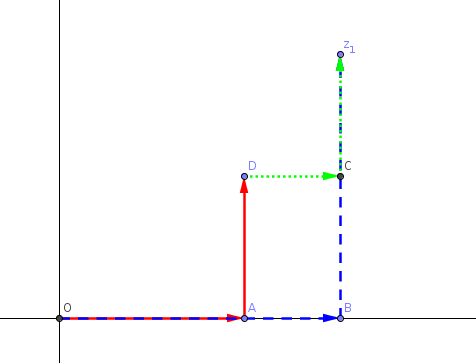
\includegraphics[width=0.5\textwidth]{immagini/percorsi-integrale.png}
\end{figure}

Adesso invece valutiamo $F(z_1)=F(z+h)$ con $h \in \C$; sulla falsa riga dell'esempio precedente, seguiamo il percorso blu ottenendo:
$$F(z+h)=\int_O ^B f(z)dz + \int_B ^{z+h} f(z')dz'$$
Applicando il teorema dei rettangoli a $\mathfrak{R}_{ABCD}$, otteniamo che la somma degli integrali sui lati del rettangolo è nulla, cioè $\int_A ^B f(z)dz+\int_B ^C f(z)dz+\int_C ^D f(z)dz+\int_D ^A f(z)dz=0$; quindi possiamo affermare che  $\int_A ^B f(z)dz+\int_B ^C f(z)dz=\int_C ^D -f(z)dz+\int_A ^D f(z)dz$. Sostituendo nella formula precedente, otteniamo che $F(z+h)=F(z)+\int_{z \to C \to z+h} f(z')dz'$.

A questo punto, facciamo in modo che sia a destra sia a sinistra appaia un rapporto incrementale; definito $\varphi$ il cammino $z \to C \to z+h$, la nostra equazione diventa:
$$\frac{F(z+h)-F(z)}{h}-f(z)=\frac{1}{h} \int_{\varphi}f(z')dz' -  f(z)\frac{1}{h} \int_{\varphi}dz'$$
dove è facile dimostrare che $f(z)=f(z)\frac{1}{h} \int_{\varphi}dz'$, perchè si ha che $\int_{\varphi}dz'=h$, e dunque: 
$$\frac{1}{h} \int_{\varphi}dz'=\frac{h}{h}=1$$

Utilizzando le proprietà dell'integrale, abbiamo che:
$$\frac{F(z+h)-F(z)}{h}-f(z)=\frac{1}{h} \int_{\varphi}[f(z')-f(z)]dz'$$
Passando ai moduli :
$$\left|\frac{F(z+h)-F(z)}{h}-f(z)\right|=\left|\frac{1}{h} \int_{\varphi}[f(z')-f(z)]dz'\right| \leq \frac{1}{|h|} \sup_{z \in \varphi} |f(z')-f(z)| (|Re(h)|+|Im(h)|)$$
Per la continuità di $f(z)$, abbiamo che $|f(z')-f(z)| < \epsilon$ e per le proprietà dei numeri complessi $|Re(h)|+|Im(h)| \leq 2|h|$; quindi otteniamo:
$$\left|\frac{F(z+h)-F(z)}{h}-f(z)\right|<2 \epsilon$$
Quindi, per $h \to 0$, si ha che $|F'(z)-f(z)|< \epsilon$, cioè $F'(z)=f(z)$; abbiamo quindi dimostrato che una funzione intera ammette primitiva.
\\
Da questa dimostrazione discende un importante teorema, il teorema di Cauchy.
\begin{teorema}
sia $f(z)$ una funzione intera e $\gamma$ un cammino chiuso; allora l'integrale di f su $\gamma$ ha valore nullo, cioè $\oint_{\gamma} f(z)dz=0$.
\end{teorema}
\section{La formula di Cauchy}

Sia $f$ una funzione intera; definiamo inoltre la funzione ausiliaria:
$$g(z)=\left\{  \begin{array}{l l}    \frac{f(z)-f(z_0)}{z-z_0} & \quad z \neq z_0\\    f'(z_0) & \quad z=z_0  \end{array} \right.$$
La funzione $g(z)$ è olomorfa ovunque tranne che in $z_0$ (cioè è olomorfa su $\C \backslash \{z_0\}$) ed è continua su tutto $\C$. Data una curva chiusa $\gamma$, con $z_0 \notin \gamma$, per le proprietà dell'integrale abbiamo che $0= \oint_{\gamma} g(z') dz'=\oint_{\gamma} \frac{f(z')-f(z_0)}{z'-z_0} dz'$. Dividendo per $2 \pi i$ otteniamo la cosiddetta formula integrale di Cauchy:
$$\oint_{\gamma} \frac{f(z')-f(z_0)}{z'-z_0} \frac{dz'}{2 \pi i} =f(z_0) Ind(\gamma, z_0)$$
Questa funzione mi permette, conoscendone i valori sulla curva $\gamma$, di conoscere i valori della funzione stessa all'interno della curva.

Sia ad esempio $\gamma$ la circonferenza centrata in $z_0$ e di raggio $\rho$; una possibile parametrizzazione è $z(\theta)=z_0 + \rho e^{i\theta}$. Inserendo nella formula ricavata precedentemente la variabile $z(\theta)$, e ricordando che il differenziale cambia ($dz=i \rho e^{i\theta}d\theta$), otteniamo:
$$i \rho  \int_0 ^{2 \pi} \frac{e^{i\theta}}{2 i \pi} \frac{f(z_0+ \rho e^{i \theta})}{ \rho  e^{i\theta}} d\theta=f(z_0)$$
Un corollario importante alla formula integrale di Cauchy è il teorema della media:
\begin{teorema}
Il valore di una funzione intera $f(z)$ al centro di una circonferenza $C_{\rho} (z_0)$ è uguale alla media (sugli angoli) dei punti sul bordo della circonferenza.
$$f(z_0)=\frac{1}{2 \pi} \int_0 ^{2 \pi} f(z_0 +  \rho e^{i\theta}) d\theta$$
\end{teorema}
\begin{corollario}
Il modulo di una funzione intera non ha picchi, cioè $|f(z_0)| \leq \sup_{|z-z_0| \leq  \rho } |f(z)|$
\end{corollario}
\begin{teorema} (di Liouville)\\
Sia $f$ una funzione intera tale che $|f(z)| \leq M$, con M finito. allora $f$ è una funzione costante. (Oppure: una funzione intera, a meno che non è costante, non è limitata in modulo).
\end{teorema}
\begin{proof}
Sfruttando la formula integrale di Cauchy, abbiamo che 
$$f(z)-f(0)=\int_{\gamma} \frac{f(z')}{z'-z} \frac{dz'}{2 \pi i}-\int_{\gamma} \frac{f(z')}{z'-0} \frac{dz'}{2 \pi i}=\int_{\gamma} \frac{z}{(z'-z)z} f(z') \frac{dz'}{2 \pi i}$$
Prendiamo come curva la circonferenza centrata nell'origine e di raggio $\rho$ tale che $|z| \leq \rho$; parametrizziamo la circonferenza come al solito: $z'=\rho e^{i\theta}$ (e quindi $dz'=i \rho e^{i\theta} d\theta$). Sostituendo nell'equazione precedente, otteniamo che:
$$f(z)-f(0)=i \rho z \int f(\rho e^{i\theta}) \frac{1}{(\rho e^{i\theta}-z)\rho e^{i\theta}} \frac{e^{i\theta}}{2 i \pi} d\theta$$
e, passando ai moduli:
$$|f(z)-f(0)|=|z| \, \left|\int f(\rho e^{i\theta}) \frac{1}{(\rho e^{i\theta}-z)\rho e^{i\theta}} \frac{e^{i\theta}}{2 i \pi} d\theta \right| \leq$$
$$\leq |z|\sup_{\theta \in [0;2\pi]} \frac{|f(\rho e^{i\theta})|}{|\rho e^{i\theta}-z|} \frac{L(\gamma)}{2 \pi} \leq$$
$$\leq |z| M \sup_{\theta \in [0;2\pi]} \frac{1}{|\rho e^{i\theta}-z|} =M \frac {|z|}{\rho-|z|}$$
Dato che possiamo prendere la circonferenza grande a piacere, mandiamo $\rho$ a $+\infty$ e quindi otteniamo che $|f(z)-f(0)| \leq 0$, ma allora, dato che il modulo è una quantità positiva, abbiamo che $|f(z)-f(0)|=0$, e quindi $f(z)=f(0)$.

\end{proof}
\begin{corollario}
Sia $f$ una funzione intera; se la funzione si annulla per $z \to \infty$, allora $f \equiv 0$.
\end{corollario}
\begin{corollario}
Se $f = \sum \alpha z^n$ per $z \to \infty$, allora $f(z)$ è un polinomio di grado $n$.
\end{corollario}
\begin{teorema} (di Picard)\\
Sia $f$ intera. Se $f(z) \neq a$ e $f(z) \neq b$, allora $f$ è costante.
\end{teorema}
Quindi l'immagine di una funzione intera è tutto il piano complesso tranne al più un punto, altrimenti la funzione è una funzione costante.
\begin{teorema} (Teorema fondamentale dell'algebra)\\
Sia $p(z)$ un polinomio di grado $n$; tale polinomio possiede almeno uno zero.
\end{teorema}
La dimostrazione di questo teorema è sufficiente per dimostrare la fattorizzazione di un polinomio.
\begin{proof}
Per assurdo, sia $p(z) \neq 0$ $\forall z$; allora $\frac{1}{p(z)}$ è intero, e si ha che $\frac{1}{p(z)} \to 0$ per $z \to 0$; infatti, dato che $p(z) \neq 0$, non può essere diverso da un'altro valore (per il teorema di Picard) e quindi $p(z)$ non è limitato. Ma allora, per il teorema di Liouville, si ha che $\frac{1}{p(z)}=0$ ovunque. il che è contro l'ipotesi di partenza. Abbiamo quindi dimostrato la tesi.
\end{proof}

Introduciamo ora la formula di fattorizzazione, che si rivelerà molto utile per il calcolo degli integrali:
\begin{equation}
p(z)=\sum_{k=1} ^n \frac{1}{p'(z_k)} \frac{1}{z-z_k}
\end{equation}
Sia ora $p(z)$ un polinomio e $\gamma$ un cammino chiuso. Il valore di $\oint_{\gamma} \frac{p'(z)}{p(z)-c} \frac{dz}{2 i \pi} $ mi dà il numero di soluzioni dell'equazione $p(z)=c$ chiuse dalla curva $\gamma$ (contate con la loro molteplicità algebrica). Come lo vediamo? \\ Chiamiamo $q(z)=p(z)-C$; tale polinomio è tale che $q'(z)=p'(z)$. sostituendo all'interno dell'integrale, otteniamo:
$$\oint_{\gamma} \frac{q'(z)}{q(z)} \frac{dz}{2 i \pi}=\oint_{\gamma} \sum_{k=1} ^n \frac{1}{z-z_k} \frac{dz}{2 i \pi}$$
dove i $z_k$ sono gli zeri di $q(z)$.
Quindi abbiamo una somma funzioni indice, cioè $\sum_k Ind(\gamma,z_k)$.

Prendiamo una funzione f continua su $\C$. Diciamo che f è doppiamente periodica se $\exists w_1,w_2 \in \C$, con $w_1 \neq \lambda w_2$ (per $\lambda \in \R$) tali che $f(z+w_1)=f(z)=f(z+w_2)$ $\forall z$, oppure in alternativa, tali che $f(z+n_1w_1+n_2w_2)=f(z)$ $\forall n_2, n_2 \in \Z$, $\forall z \in \C$.
\begin{teorema} (di Dixon)\\
Sia $\mathcal{D}$ aperto e connesso, $\gamma$ cammino differenziabile con continuità  a tratti, $Ind(\gamma,z)=0$ $\forall z \in \mathcal{D}$, f funzione olomorfa su $\mathcal{D}$. Allora valgono le formule delle funzioni intere, cioè:
$$\int_{\gamma} f(z') dz'=0 \text{ e } \int_{\gamma} \frac{f(z')}{z-z'} \frac{dz'}{2 \pi i}=f(z) Ind(\gamma,z)$$
con $z \notin \gamma$.
\end{teorema}
Vale anche il teorema inverso:
\begin{teorema} (di Morera)\\
Se l'integrale di Cauchy di una funzione continua si annulla per tutti i cammini chiusi (differenziabili con continuità a tratti) in un dominio limitato $\mathcal{D}$, allora $f$ è olomorfa su $\mathcal{D}$.
\end{teorema}

\section{La funzione Gamma di Eulero}

La funzione Gamma di Eulero è definita come:

\begin{equation}
\Gamma (z)= \int_0 ^{\infty} e^{-s} s^{z-1} ds
\end{equation}
dove s è un numero complesso; questo ci permette di riscrivere $\Gamma (z)$ come:
$$\Gamma (z)=\int_0 ^{\infty} e^{-s} s^{x-1} e^{iy log(s)} ds$$
In questo modo, risulta ovvio che:
$$|\Gamma (z)| \leq \int_0 ^{\infty} e^{-s} s^{x-1} ds = \Gamma (Re(z))$$
Quindi si ha che in $Re(z)>0$ la funzione $\Gamma(z)$ è olomorfa. Le principali proprietà della Gamma di Eulero sono:
\begin{itemize}
\item $\int_{\gamma} \Gamma (z) dz=\int_{\gamma} dz \int_0 ^{\infty} e^{-s} s^{z-1} ds= \int_0 ^{\infty} e^{-s} \int_{\gamma} e^{(z-1)log(s)} dz ds=0$
\item $\Gamma (x+1) = x \Gamma (x)$
\item $\Gamma (1)=1$ e, per induzione, $\Gamma (n+1)=n!$
\item $\Gamma (\frac{1}{2}) = \sqrt{\pi}$
\item $\Gamma (n+ \frac{1}{2})= \frac{2n-1}{2} \Gamma (\frac{1}{2})= \frac{(2n-1)}{2} \sqrt{\pi}$
\end{itemize}

